\documentclass[aps,pra,groupedaddress,onecolumn,notitlepage,superscriptaddress,10pt]{revtex4-1}

%\usepackage[utf8]{inputenc}
%\usepackage{mathpazo}
%\usepackage{mathptmx}
%\usepackage{tgpagella}
%\usepackage{tgtermes}

\usepackage{float}
\usepackage{graphicx}  % needed for figures
\usepackage{xcolor}
\usepackage{dcolumn}   % needed for some tables
\usepackage{bm}        % for math
\usepackage{braket}
\usepackage{amssymb}   % for math
\usepackage{epstopdf}
\usepackage{xfrac}

\usepackage{amsmath}
\usepackage{amsthm}
\usepackage{amsfonts}
\usepackage{bbm}
% configure hyperref to remove ugly boxes from links
\definecolor{darkblue}{rgb}{0.1,0.2,0.6}
\definecolor{darkred}{rgb}{0.8,0.1,0.2}
\usepackage[colorlinks,citecolor=darkblue,linkcolor=darkblue,urlcolor=darkblue]{hyperref} 
\usepackage{tikz}
\usepackage{enumerate}
\usepackage{setspace}
\usepackage{url}  % This makes \url work
\usepackage{mathrsfs}

\def\ua{\uparrow}
\def\da{\downarrow}
\newcommand{\rT}{{\rho^{T_2}} }
\newcommand{\rTa}{{\rho^{T_2}_A} }
\newcommand{\rTc}{{\rho^{T_2}} }
\newcommand{\Hi}{\mathcal{H}}
\newcommand{\Ni}{\mathcal{N}}
\newcommand{\C}{\mathbb{C}}
\newcommand{\Z}{\mathbb{Z}}
\newcommand{\R}{\mathbb{R}}
\newcommand{\I}{\mathbb{I}}
\newcommand{\Rp}{{\cal R}_\text{part}}
\newcommand{\sgn}{\text{sign}}

\newcommand{\xv}{\textbf{x}}
\newcommand{\ev}{\textbf{e}}
\newcommand{\iv}{\textbf{i}}
\newcommand{\jv}{\textbf{j}}
\newcommand{\Tr}{\text{Tr}}
\newcommand{\tr}{\text{Tr}}
\newcommand{\del}{\nabla}
\newcommand{\norm}[1]{\left\lVert#1\right\rVert}

\newcommand{\vac}{\ket{0}\bra{0}}
\newcommand{\kvac}{\ket{\text{vac}}}
\newcommand{\bvac}{\bra{\text{vac}}}
\newcommand{\bigket}[1]{ {\big|{#1}\big\rangle} }
\newcommand{\Bigket}[1]{ {\Big|{#1}\Big\rangle} }
\newcommand{\bigbra}[1]{ {\big\langle{#1}\big|} }
\newcommand{\Bigbra}[1]{ {\Big\langle{#1}\Big|} }


\usepackage{tikz}
\usetikzlibrary{positioning}
\usetikzlibrary{patterns}

%\usepackage{tikzit}

\newcommand*{\HS}[1]{\textcolor{blue}{[HS: #1]}}
\newcommand*{\SL}[1]{\textcolor{magenta}{[SL: \textsf{#1}]}}
\newcommand*{\change}[2]{{\color{red}\sout{#1}}{ \color{blue}#2}}

\begin{document}

\title{Entanglement transitions in random pure states}
\author{Hassan Shapourian%
%  \thanks{Electronic address: \texttt{hassan.shapp@gmail.com}}
  }
\affiliation{Microsoft Station Q, Santa Barbara, CA 93106, USA}
% \affiliation{Department of Physics, Harvard University, Cambridge, MA~02138, USA}
% \affiliation{Department of Physics, Massachusetts Institute of Technology,
% Cambridge, MA~02139, USA}
\author{Jonah Kudler-flam}
\affiliation{Kadanoff Center for Theoretical Physics, University of Chicago, IL 60637, USA}


\date{\today}

\begin{abstract}
In this paper, we use large-$N$ perturbation theory to compute the entanglement negativity of random induced mixed states. Our result reproduces the two well-known limits: volume law states and separable states. We also find that the volume law states can be further divided into two categories in terms of subsystem-size scaling  of the entanglement  negativity: a linear scaling phase, where the state is maximally entangled and the logarithmic negativity is bound by the size of the smaller subsystem ${\cal E}\sim V_{A_1}$, and a saturated phase, where ${\cal E}\sim (V_{A}-V_B)/2$, which  is independent of individual subsystem sizes $V_{A_1}$ and $V_{A_2}$. In the latter case, the spectral density can be well-approximated by a semi-circle law. We show that the large-$N$ perturbation theory results match with those of the random matrix simulations.
Our finding indicates that the average logarithmic negativity behaves very similar to the $1/2$-R\'enyi mutual information.
\end{abstract}

\maketitle

\section{Introduction}

Random pure states represent typical volume law entangled  (thermal) pure states. Their virtue is that they are described by Wishart random matrix theory and hence, various well-established random matrix theory tools are available to carry out calculations on them.

In this paper, we use the large-N perturbation theory which was recently developed by one of us~\cite{SLA20} to compute the spectral density of partial transpose and characterize the reduced density matrix in several limits. The result is summarized in Fig.~\ref{fig:phasediag}.


\begin{figure}
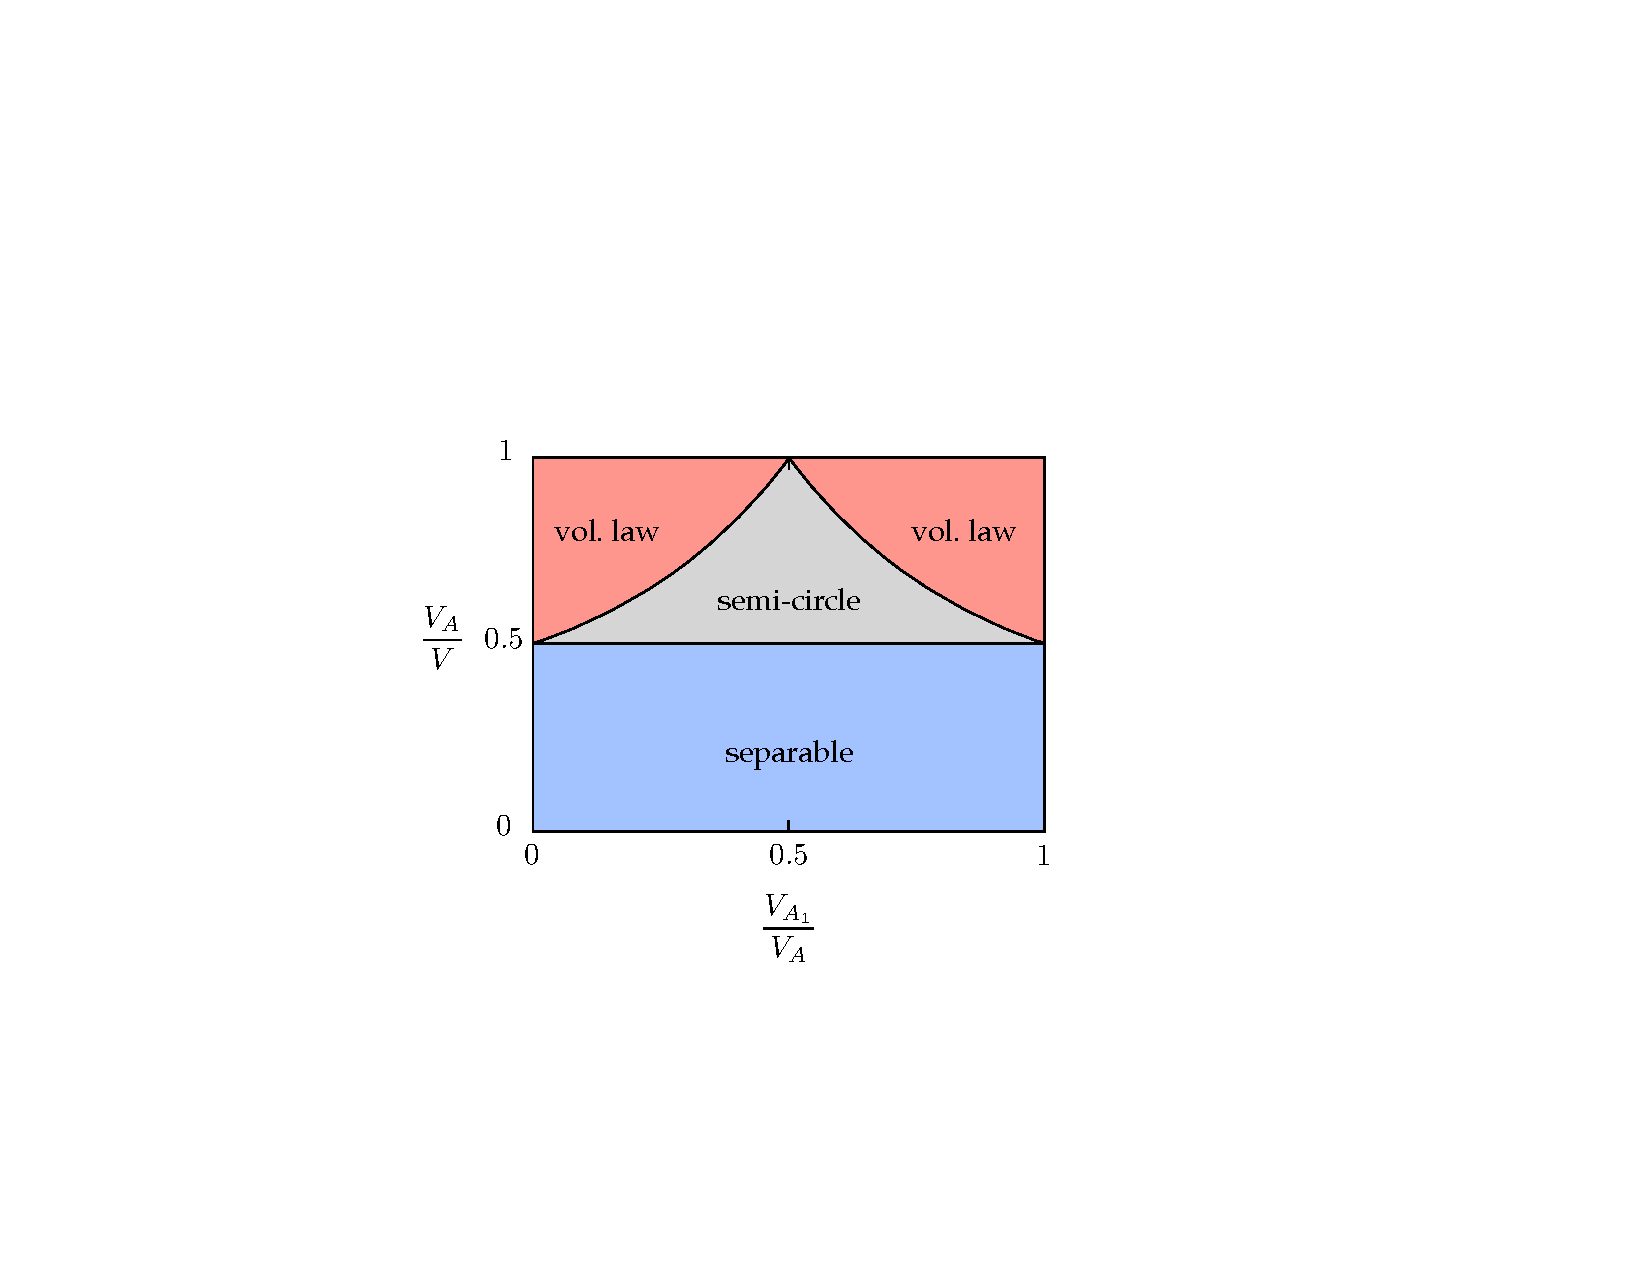
\includegraphics[scale=0.6]{images/phase_diag.pdf}
\caption{\label{fig:phasediag} Phase diagram of reduced density matrix obtained from random pure states (or Page states).}
\end{figure}


We would like to study the entanglement in random mixed states obtained by partial tracing over random pure states.  Concretely, consider a random pure state, aka Page state (or Haar state),  $\ket{\Psi}$ in a composite Hilbert space $\Hi= \Hi_{A}\otimes \Hi_{B}$. Here, the word random means uniformly distributed on the sphere of the Hilbert space $\Hi$.
An ensemble of reduced density matrices $\{ \rho \}$ acting on the Hilbert space $\Hi_A=\Hi_{A_1}\otimes \Hi_{A_2}$ is generated by  $\rho_A=\Tr\ket{\Psi}\bra{\Psi}$.
It is more convenient to represent such a random pure state in
a tensor product basis as in
\begin{align}
\label{eq:page_tri}
\ket{\Psi}=\sum_{i=1}^{L_A} \sum_{\alpha=1}^{L_B} X_{i\alpha} \ |\Psi^{(i)}_{A} \rangle\otimes|\Psi^{(\alpha)}_B\rangle,
\end{align}
in terms of a $L_A \times L_B$ rectangular random matrix $X$
whose elements ($X_{i \alpha}$) are independent random complex variables. Here, $L_{A}=L_{A_1}\times L_{A_2}$ and $L_B$ denote the size of $\Hi_A$ and $\Hi_B$, respectively. Throughout this paper, we consider $A$ and $B$ systems to be comprised of qubits. In other words,  $L_s=2^{V_s}$ where $s=A_1,A_2,B$ and $V_s$ is the number of qubits. This choice is not a necessary ingredient for our calculations and is mainly meant as a physical description of the system.

By definition, the joint probability density is given by
\begin{align}
    \label{eq:Xprob}
    P\left( \{X_{i\alpha} \} \right) = {\cal Z}^{-1} \exp \left\{- L_A L_B \Tr(XX^\dag) \right\}.
\end{align}
The random reduced density matrix of system $A$ is then given by
\begin{align}
\label{eq:red_den}
\rho_{A}=\frac{XX^{\dag}}{\tr (X X^\dag)}.
\end{align}
We note that $\rho_A$ is a $L_A \times L_A$ square matrix, and  the denominator (which is also a random variable) is there to enforce the normalization condition $\Tr \rho_A=1$.


The eigenvalues of $\rho_A$ (aka the entanglement spectrum) contains information about the entanglement between $A$ and $B$. In the limit $L_A, L_B \to \infty$ while the ratio $L_A/L_B$ is finite (which we will refer to as the large $L$ limit from now on), 
the joint probability density function of these eigenvalues can be derived~\cite{Lloyd1988, Zyczkowski2001}. In doing so, the crucial approximation is that the normalization factor in Eq.~(\ref{eq:red_den}) is a random variable $\Tr (XX^\dag)= 1+ \delta$ whose fluctuations about its mean $1$ is negligible to the leading order in $L_A L_B$. Hence, to the leading order, the denominator can be approximated by its mean value, and we may write
\begin{align}
% \rho_A \approx \frac{XX^\dag}{ L_A L_B}.
 \rho_A \approx XX^\dag.
 \label{eq:Wishart}
\end{align}
 which is the celebrated  Wishart-Laguerre ensemble~\cite{Forrester} and is extensively studied in the random matrix theory literature. From this observation, one can infer several properties of $\rho_A$ in the large $L$ limit. Among all, the spectral density of the eigenvalues is given by an appropriately scaled Marcenko-Pastur (MP) function \cite{Forrester}. In the following sections, we present a graphical representation for $\rho_A$ and its partial transpose $\rho_A^{T_2}$ which will be used to calculate the spectral density of eigenvalues of $\rT$.

\section{Large-N perturbation theory}
In this section, we use graphical representation of a partially transposed random mixed state to  compute its momets  and eventually derive the corresponding resolvent function and the spectral density.

We begin by reviewing the diagrammatic approach to random pure states~\cite{Jurkiewicz,Zee1995}. This method is based on the `t~Hooft $1/N$ (double line) perturbation theory which was also used recently in the context of black hole information problems~\cite{Shenker2019}.

A matrix element of the pure state density matrix (\ref{eq:page_tri}) is denoted as
\begin{align}
    \left[\ket{\Psi}\bra{\Psi}\right]_{i\alpha,j\beta}= X_{i\alpha}^\ast X_{j\beta}
    =%\frac{1}{\cal N} \
    \,
    \tikz[baseline=-0.5ex]{
    \draw[dashed] (0,0.2) node[align=center, above] {\footnotesize $\alpha$} -- (0,-0.2);
    \draw[dashed] (1,0.2) node[align=center, above] {\footnotesize $\beta$} -- (1,-0.2);
    \draw[line width=2] (-0.2,0.2) node[align=center, above] {\footnotesize $i$} -- (-0.2,-0.15);
    \draw[line width=2] (1.2,0.2) node[align=center, above] {\footnotesize $j$} -- (1.2,-0.15);
    % \node[draw,text width=4cm] at (2,-2) {i};
    }\ ,
\end{align}
where the left (right) pair of lines represents a bra (ket) state, and solid (dashed) lines correspond to subsystem $A$ ($B$). Note that each line carries an index. The lower end of the diagrams are reserved for matrix manipulations such as tracing and multiplication, while the upper ends of the lines are used for ensemble averaging.
Hence, a matrix element of the reduced density matrix is represented by
\begin{align}
    \label{eq:rho_diag}
    [\rho_A]_{i,j}= 
    %{\cal N}^{-1}\,
    {\sum_{\alpha=1}^{L_B} X_{i\alpha}^\ast X_{j\alpha}}
= %\frac{1}{\cal N} \
\,
    \tikz[baseline=-0.5ex]{
    \draw[dashed] (0,0.2) node[align=center, above] {\footnotesize $\alpha$} -- (0,0);
    \draw[dashed] (0,0)  -- (1,0);
    \draw[dashed]  (1,0.2) node[align=center, above] {\footnotesize $\alpha$} -- (1,0);
    \draw[line width=2] (-0.2,0.2) node[align=center, above] {\footnotesize $i$} -- (-0.2,-0.15);
    \draw[line width=2] (1.2,0.2) node[align=center, above] {\footnotesize $j$} -- (1.2,-0.15);
    }\ .
\end{align}
For brevity, from now on we drop the subscript $A$ in $\rho_A$ unless stated otherwise.
Moreover, ensemble averaging is achieved by connecting the upper terminals by
\begin{align}
\braket{X_{i \alpha} H_{j \beta}} \equiv
\
\tikz[baseline=-0.8ex,scale=1]{
    \draw[line width=2] (0,-0.05)--(1.1,-0.05);
    \draw[dashed] (0,-0.2)--(1.1,-0.2);
    }
    \ 
    =\frac{1}{L_{A} L_B}\, \delta_{i_1 j_1} \delta_{i_2 j_2} \delta_{\alpha\beta}.
\end{align} 
For instance, the normalization condition on average is represented by the diagram,
For example, we may write
\begin{align}
    \braket{\Tr\rho}=
    %\frac{1}{\cal N} \ 
    \,
    \tikz[baseline=0ex]{
    %\draw[dashed] (0,0) .. controls (0.25,0.8) and (0.75,0.8) .. (1,0) ;
    \draw[dashed] (1.0,0) arc (0:180:0.5);
    \draw[dashed] (0,0) -- (1,0);
    \draw[line width=2] (1.2,0.) arc (0:180:0.7);
    \draw[line width=2] (-0.2,0.0)-- (-0.2,-0.15)--(1.2,-0.15)-- (1.2,0.0);
    }\ = 1.
\end{align}

We now incorporate the partial transpose as an operation on the density matrix (\ref{eq:rho_diag}).
First, we note that we need a tri-partite geometry; in other words, subsystem $A$ is further partitioned into $A_1$ and $A_2$. So, we define a (more refined) bipartite reduced density matrix by
\begin{align}
    [\rho]_{i_1i_2,j_1j_2}= \sum_\alpha X^\ast_{(i_1i_2),\alpha}X_{(j_1j_2),\alpha}
    =
    %\frac{1}{{\cal Z}} \ 
    \,
    \tikz[scale=0.8,baseline=-0.5ex]{
    \draw[dashed] (0,0.2)-- (0,0);
    \draw[dashed] (0,0) -- (1,0);
    \draw[dashed]  (1,0.2) -- (1,0);
    \draw (-0.2,0.2)-- (-0.2,-0.15);
    \draw (1.2,-0.15)-- (1.2,0.2);
    \draw[densely dotted,thick] (-0.3,0.2)-- (-0.3,-0.15);
    \draw[densely dotted,thick] (1.3,-0.15)-- (1.3,0.2);
    }\ ,
\end{align}
where the dotted and solid lines correspond to subsystems $A_1$ and $A_2$, respectively. 
Partial transpose is diagrammatically shown as
\begin{align}
	\label{eq:rT_diag}
    [\rho^{T_2}]_{i_1i_2,j_1j_2}= \sum_\alpha X^\ast_{(i_1\textcolor{red}{j_2}),\alpha}X_{(j_1\textcolor{red}{i_2}),\alpha}
    %\frac{1}{\cal Z} \ 
    =\,
    \tikz[scale=0.8,baseline=-1.5ex]{
    \draw[dashed] (0,0.2)-- (0,0);
    \draw[dashed] (0,0) -- (1,0);
    \draw[dashed]  (1,0.2) -- (1,0);
    \draw (-0.2,0.2)-- (-0.2,-0.15);
    \draw (-0.2,-0.15)-- (1.,-0.7);
    \draw (1.2,-0.15)-- (1.2,0.2);
    \draw (1.2,-0.15)-- (0,-0.7);
    \draw[densely dotted,thick] (-0.3,0.2)-- (-0.3,-0.4);
%    \draw[densely dotted,thick] (-0.3,-0.4)-- (1.3,-0.4);
    \draw[densely dotted,thick] (1.3,-0.4)-- (1.3,0.2);
    }\ .
\end{align}
The underlying operation in the above diagram is to swap the indices for one subsystem as emphasized by indices highlighted in red. Such implementation of the partial transpose is indeed not limited to random density matrices and can be applied to deterministic density matrices of spin chains. In the latter context, we need to impose certain rules on the diagrammatic representation of the partial transpose to make it consistent with time-reversal symmetry. For instance, Penrose diagrams~\cite{1996PhRvD..54.2664D,Rovelli:2004tv}
provides such a consistent representation which can be used  to derive the $Z_2$ topological invariant for topological phases of spin chains protected by time-reversal symmetry~\cite{SMR20}.

One can easily check that the above definition of partial transpose is trace preserving and does not change the purity, i.e. $\Tr\rT^2=\Tr\rho^2$.

\subsection{Moments of partial transpose}


Let us look at the dominant diagrams deep in the NPT limit, $L_A\gg L_B$, when one subsystem ($A_1$ or $A_2$) is much larger than the other. 
\begin{align}
    \braket{\Tr \left(\rho^{T_2}\right)^{n_e} } \approx \ 
    \left\{
    \begin{matrix}
    L_{B}^{1-n_e} L_{A_2}^{2-n_e} & \qquad  L_{A_1} \gg L_{A_2}
    \\
    \\
    L_{B}^{1-n_e} L_{A_1}^{2-n_e} & \qquad  L_{A_1} \ll L_{A_2}
    \end{matrix}
    \right.
\end{align}

\begin{align}
    &
    \vcenter{\hbox{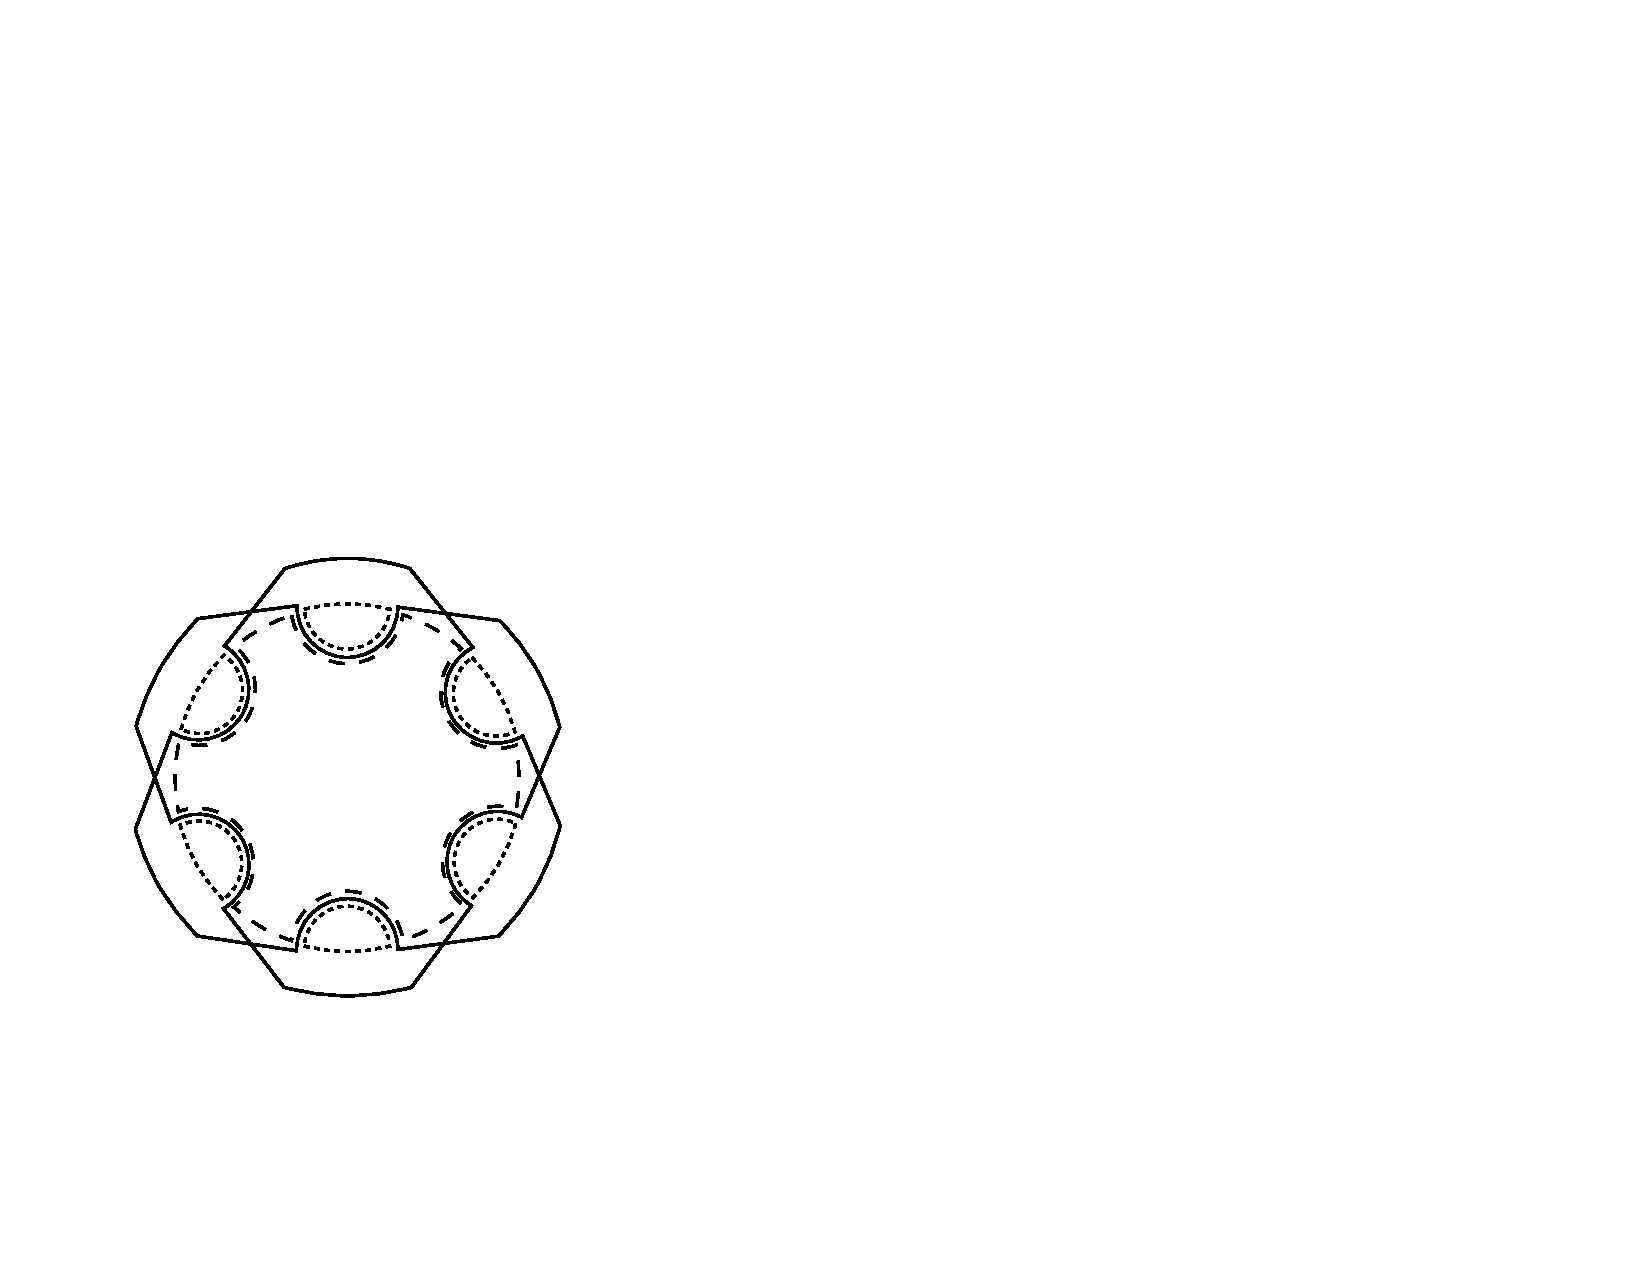
\includegraphics[scale=0.4]{images/RN6_A1large.pdf}}},
\end{align}
\begin{align}
    \vcenter{\hbox{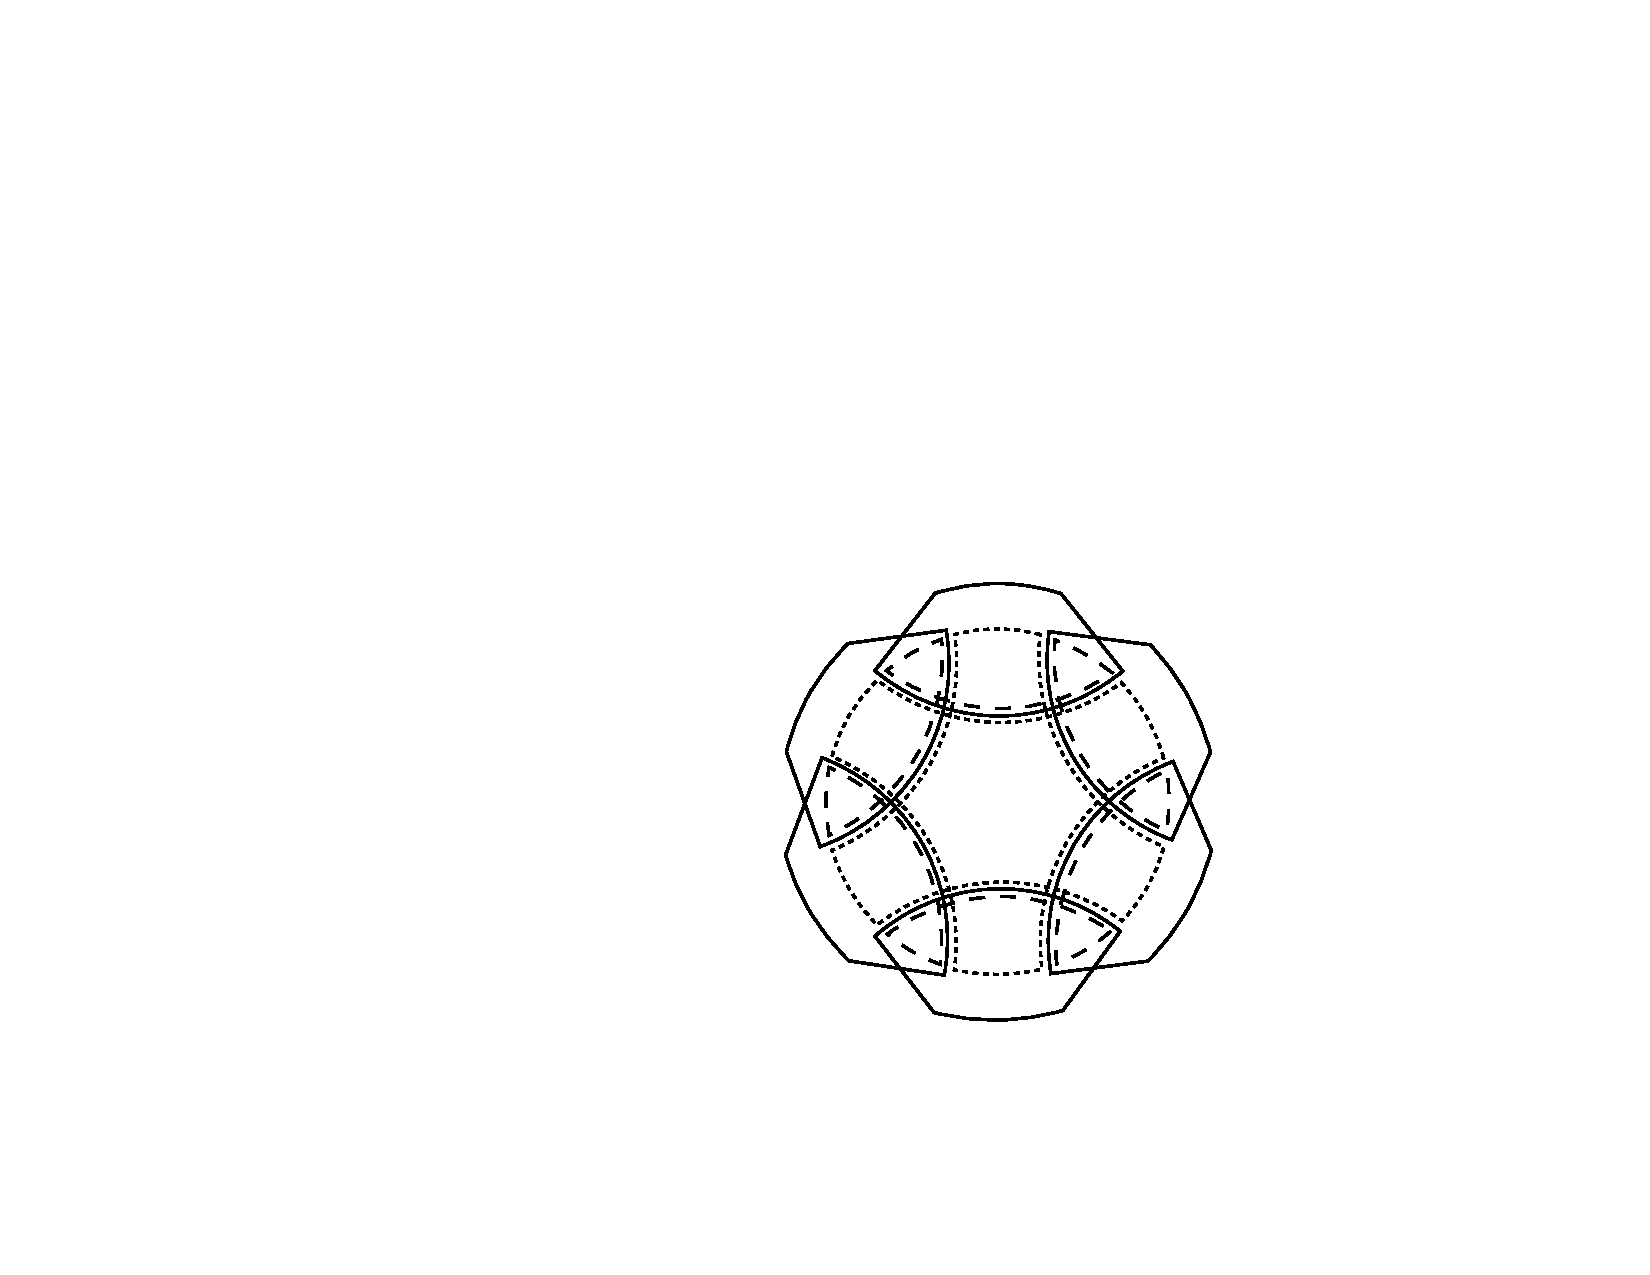
\includegraphics[scale=0.4]{images/RN6_A2large.pdf}}},
\end{align}
TMD spacetime conjecture vs RMT (assuming $L_{A_1}\gg L_{A_2}$):
\begin{align}
	\braket{\Tr \left(\rho^{T_2}\right)^n } \approx \ 
    \left\{
    \begin{matrix}
    \text{genus}~k~\text{with}~1\times \text{puncture}
    & 
    &
    n\times A_1,   1\times A_2, 1\times B 
     & \qquad  n=2k+1
    \\
    \\
    \text{genus}~(k-1)~\text{with}~2\times \text{punctures}
    & 
    &
    n\times A_1,   2\times A_2, 1\times B 
     & \qquad  n=2k
    \end{matrix}
    \right.
\end{align}


This suggests that
\begin{align}
    \braket{\cal E} \approx \ 
    \left\{
    \begin{matrix}
    \log L_{A_2} & \qquad  L_{A_1} \gg L_{A_2},
    \\
    \\
    \log L_{A_1} & \qquad  L_{A_1} \ll L_{A_2}.
    \end{matrix}
    \right.
\end{align}
This analysis may have some issues such as dependence on how we analytically continue R\'enyi index.
In the next part, we use the resolvent function to calculate the spectral density of $\rT$ which provides an unambiguos way to derive the logarithmic negativity.



\subsection{Resolvent function}

Our goal in this part is to derive the spectral density of the partially transposed density matrix.
To this end, we define a one-point Green function (or a resolvent function) as
\begin{align}
    G(z)=\frac{1}{L_A} \left\langle \Tr\left( \frac{1}{z-H}\right) \right\rangle,
\end{align}
where we use a particular normalization and define $H=L_B L_{A_2} (XX^\dag)^{T_2}$ to carry out calculations systematically such that $1/N$ perturbative expansion makes sense. 
The actual normalization will be included via rescaling after the spectral density is evaluated. We can then compute the spectral density using the identity
\begin{align}
    \label{eq:dos}
    P_\Gamma(\xi)= - \frac{L_A}{\pi} \text{Im} \lim_{\epsilon\to 0} G(z)\big|
    _{z=\xi + i\epsilon},
\end{align}
because
\begin{align}
    \lim_{\epsilon\to 0} \frac{1}{\lambda + i\epsilon} = \text{PV}\, \frac{1}{\lambda} - i \pi \delta(\lambda).
\end{align}
The Feynman diagram approach follows by expanding $G(z)$ in inverse powers of $z$. In our graphical representation of a given term, we insert the diagram (\ref{eq:rT_diag}) for every power of $\rTc$. 
The ensemble average is represented by triple lines with amplitude $1/L_{A_1}$ (given the above normalization),
\begin{align}
\braket{H_{i_1 j_1 \alpha} H_{i_2 j_2 \beta}} \equiv
\
\tikz[baseline=-0.8ex,scale=1]{
    \draw[densely dotted,thick] (0,0.05)--(1.1,0.05);
    \draw (0,-0.05)--(1.1,-0.05);
    \draw[dashed] (0,-0.2)--(1.1,-0.2);
    }
    \ 
    =\frac{1}{L_{A_1}}\, \delta_{i_1 j_1} \delta_{i_2 j_2} \delta_{\alpha\beta},
\end{align} 
and as usual close loop of subsystem $s=A_1,A_2$, or $B$ gives a factor of $L_s$.

We note that since there is an even/odd effect for the R\'enyi negativity, we need to consider two self-energy functions in the expansion of the resolvent function
\begin{align}
    \tikz[baseline=-0.5ex]{
    \draw[densely dotted,thick] (0.35,0.05)--(0.65,0.05);
    \draw[densely dotted,thick] (-0.35,0.05)--(-0.65,0.05);
    \draw (0.35,-0.05)--(0.65,-0.05);
    \draw (-0.35,-0.05)--(-0.65,-0.05);
    \draw[thick] (0,0) circle (10pt) node[anchor=center] {$G$};
    }
    =&
   \tikz[baseline=-0.5ex]{
    \draw[densely dotted,thick] (-0.4,0.05)--(0.35,0.05);
    \draw (-0.4,-0.05)--(0.35,-0.05);
    }
    +
    \tikz[baseline=-0.5ex]{
    \draw[densely dotted,thick] (0.35,0.05)--(0.65,0.05);
    \draw[densely dotted,thick] (-0.35,0.05)--(-0.65,0.05);
    \draw (0.35,-0.05)--(0.65,-0.05);
    \draw (-0.35,-0.05)--(-0.65,-0.05);
    \draw[thick] (0,0) circle (10pt) node[anchor=center] {$\Sigma_o$};
    }
    +
    \tikz[baseline=-0.5ex]{
    \draw[densely dotted,thick] (0.35,0.05)--(0.65,0.05);
    \draw[densely dotted,thick] (-0.35,0.05)--(-0.65,0.05);
    \draw (0.35,-0.05)--(0.65,-0.05);
    \draw (-0.35,-0.05)--(-0.65,-0.05);
    \draw[thick] (0,0) circle (10pt) node[anchor=center] {$\Sigma_e$};
    }
    \nonumber \\
    &+
    \tikz[baseline=-0.5ex]{
    \draw[densely dotted,thick] (0.35,0.05)--(0.65,0.05);
    \draw[densely dotted,thick] (-0.35,0.05)--(-0.65,0.05);
    \draw (0.35,-0.05)--(0.65,-0.05);
    \draw (-0.35,-0.05)--(-0.65,-0.05);
    \draw[thick] (0,0) circle (10pt) node[anchor=center] {$\Sigma_o$};
    \draw[thick] (1.05,0) circle (10pt) node[anchor=center] {$\Sigma_e$};
    \draw[densely dotted,thick] (1.4,0.05)--(1.7,0.05);
    \draw (1.4,-0.05)--(1.7,-0.05);
    }
+
   \tikz[baseline=-0.5ex]{
    \draw[densely dotted,thick] (0.35,0.05)--(0.65,0.05);
    \draw[densely dotted,thick] (-0.35,0.05)--(-0.65,0.05);
    \draw (0.35,-0.05)--(0.65,-0.05);
    \draw (-0.35,-0.05)--(-0.65,-0.05);
    \draw[thick] (0,0) circle (10pt) node[anchor=center] {$\Sigma_e$};
    \draw[thick] (1.05,0) circle (10pt) node[anchor=center] {$\Sigma_o$};
    \draw[densely dotted,thick] (1.4,0.05)--(1.7,0.05);
    \draw (1.4,-0.05)--(1.7,-0.05);
    }
    + \cdots \nonumber \\
      &=\frac{1}{z- \Sigma_o(z) - \Sigma_e(z)},
      \label{eq:geometric}
\end{align}
where 
\begin{align}
\tikz[baseline=-0.5ex]{
    \draw[thick] (0,0) circle (10pt) node[anchor=center] {$\Sigma_o$};
    }
=& \ \,
\tikz[scale=0.8,baseline=-1.5ex]{
    \draw[dashed] (0,0) -- (1,0);
    \draw (-0.2,0.0)-- (-0.2,-0.15);
    \draw (-0.2,-0.15)-- (1.,-0.7);
    \draw (1.2,-0.15)-- (1.2,0.0);
    \draw (1.2,-0.15)-- (0,-0.7);
    \draw[densely dotted,thick] (-0.3,0.0)-- (-0.3,-0.4);
    \draw[densely dotted,thick] (1.3,-0.4)-- (1.3,0.0);
    %%%% average
    \draw[dashed] (1,0) arc (0:180:0.5);
    \draw (1.2,0) arc (0:180:0.7);
    \draw[densely dotted,thick] (1.3,0) arc (0:180:0.8);
    }
 \ \,
+
\tikz[scale=0.5,baseline=1.5ex]{
    \draw[dashed] (0,0) -- (1,0);
    \draw (-0.2,0.)-- (-0.2,-0.15);
    \draw (-0.2,-0.15)-- (1.,-0.7);
    \draw (1.2,-0.15)-- (1.2,0.0);
    \draw (1.2,-0.15)-- (0,-0.8);
    \draw[densely dotted,thick] (-0.3,0.)-- (-0.3,-0.4);
    \draw[densely dotted,thick] (1.3,-0.1)-- (1.3,0.);
    %%%%%
    \draw[dashed] (2,0) -- (3,0);
    \draw (1.8,0.)-- (1.8,-0.15);
    \draw (1.8,-0.15)-- (3.,-0.7);
    \draw (3.2,-0.15)-- (3.2,0.);
    \draw (3.2,-0.15)-- (2,-0.7);
    \draw[densely dotted,thick] (1.7,0.)-- (1.7,-0.1);
    \draw[densely dotted,thick] (3.3,-0.1)-- (3.3,0.);
    %%%
    \draw[dashed] (4,0) -- (5,0);
    \draw (3.8,0.)-- (3.8,-0.15);
    \draw (3.8,-0.15)-- (5.,-0.8);
    \draw (5.2,-0.15)-- (5.2,0.);
    \draw (5.2,-0.15)-- (4,-0.7);
    \draw[densely dotted,thick] (3.7,0.)-- (3.7,-0.1);
    \draw[densely dotted,thick] (5.3,-0.4)-- (5.3,0.);
    %%%% contractions
    \draw[densely dotted,thick] (1.3,-0.1)--(1.7,-0.1);
    \draw[densely dotted,thick] (3.3,-0.1)--(3.7,-0.1);
    \draw (1.0,-0.7)-- (2,-0.7);
    \draw (3.0,-0.7)-- (4,-0.7);
    %%%% average
    \draw[densely dotted,thick] (5.3,0) arc (0:180:2.8);
    \draw[densely dotted,thick] (1.7,0) arc (0:180:0.2);
    \draw[densely dotted,thick] (3.7,0) arc (0:180:0.2);
    \draw[dashed] (4.0,0) arc (0:180:0.5);
    \draw[dashed] (2.0,0) arc (0:180:0.5);
    \draw[dashed] (5.0,0) arc (0:180:2.5);
    \draw (3.8,0) arc (0:180:0.3);
    \draw (1.8,0) arc (0:180:0.3);
    \draw (5.2,0) arc (0:180:2.7);
 }
 \ \,
+
\cdots,
\end{align}
%
\begin{align}
\tikz[baseline=-0.5ex]{
    \draw[thick] (0,0) circle (10pt) node[anchor=center] {$\Sigma_e$};
    }
=& \ \,
\tikz[scale=0.45,baseline=-0.5ex]{
    \draw[dashed] (0,0) -- (1,0);
    \draw (-0.2,0.)-- (-0.2,-0.15);
    \draw (-0.2,-0.15)-- (1.,-0.7);
    \draw (1.2,-0.15)-- (1.2,0.0);
    \draw (1.2,-0.15)-- (0,-0.8);
    \draw[densely dotted,thick] (-0.3,0.)-- (-0.3,-0.4);
    \draw[densely dotted,thick] (1.3,-0.1)-- (1.3,0.);
    %%%%%
    \draw[dashed] (2,0) -- (3,0);
    \draw (1.8,0.)-- (1.8,-0.15);
    \draw (1.8,-0.15)-- (3.,-0.8);
    \draw (3.2,-0.15)-- (3.2,0.);
    \draw (3.2,-0.15)-- (2,-0.7);
    \draw[densely dotted,thick] (1.7,0.)-- (1.7,-0.1);
    \draw[densely dotted,thick] (3.3,-0.4)-- (3.3,0.);
     %%%% contractions
    \draw[densely dotted,thick] (1.3,-0.1)--(1.7,-0.1);
    \draw (1.0,-0.7)-- (2,-0.7);
    %%%% average
    \draw[densely dotted,thick] (3.3,0) arc (0:180:1.8);
    \draw[densely dotted,thick] (1.7,0) arc (0:180:0.2);
    \draw[dashed] (2.0,0) arc (0:180:0.5);
    \draw[dashed] (3.0,0) arc (0:180:1.5);
    \draw (1.8,0) arc (0:180:0.3);
    \draw (3.2,0) arc (0:180:1.7);
 }
\ \,
+
\tikz[scale=0.4,baseline=1.5ex]{
    \draw[dashed] (0,0) -- (1,0);
    \draw (-0.2,0.)-- (-0.2,-0.15);
    \draw (-0.2,-0.15)-- (1.,-0.7);
    \draw (1.2,-0.15)-- (1.2,0.0);
    \draw (1.2,-0.15)-- (0,-0.8);
    \draw[densely dotted,thick] (-0.3,0.)-- (-0.3,-0.4);
    \draw[densely dotted,thick] (1.3,-0.1)-- (1.3,0.);
    %%%%%
    \draw[dashed] (2,0) -- (3,0);
    \draw (1.8,0.)-- (1.8,-0.15);
    \draw (1.8,-0.15)-- (3.,-0.7);
    \draw (3.2,-0.15)-- (3.2,0.);
    \draw (3.2,-0.15)-- (2,-0.7);
    \draw[densely dotted,thick] (1.7,0.)-- (1.7,-0.1);
    \draw[densely dotted,thick] (3.3,-0.1)-- (3.3,0.);
    %%%
    \draw[dashed] (4,0) -- (5,0);
    \draw (3.8,0.)-- (3.8,-0.15);
    \draw (3.8,-0.15)-- (5.,-0.7);
    \draw (5.2,-0.15)-- (5.2,0.);
    \draw (5.2,-0.15)-- (4,-0.7);
    \draw[densely dotted,thick] (3.7,0.)-- (3.7,-0.1);
    \draw[densely dotted,thick] (5.3,-0.1)-- (5.3,0.);
    %%%
    \draw[dashed] (6,0) -- (7,0);
    \draw (5.8,0.)-- (5.8,-0.15);
    \draw (5.8,-0.15)-- (7.,-0.8);
    \draw (7.2,-0.15)-- (7.2,0.);
    \draw (7.2,-0.15)-- (6,-0.7);
    \draw[densely dotted,thick] (5.7,0.)-- (5.7,-0.1);
    \draw[densely dotted,thick] (7.3,-0.4)-- (7.3,0.);
    %%%% contractions
    \draw[densely dotted,thick] (1.3,-0.1)--(1.7,-0.1);
    \draw[densely dotted,thick] (3.3,-0.1)--(3.7,-0.1);
    \draw[densely dotted,thick] (5.3,-0.1)--(5.7,-0.1);
    \draw (1.0,-0.7)-- (2,-0.7);
    \draw (3.0,-0.7)-- (4,-0.7);
    \draw (5.0,-0.7)-- (6,-0.7);
    %%%% average
    \draw[densely dotted,thick] (7.3,0) arc (0:180:3.8);
    \draw[densely dotted,thick] (1.7,0) arc (0:180:0.2);
    \draw[densely dotted,thick] (3.7,0) arc (0:180:0.2);
    \draw[densely dotted,thick] (5.7,0) arc (0:180:0.2);
    \draw[dashed] (6.0,0) arc (0:180:0.5);
    \draw[dashed] (4.0,0) arc (0:180:0.5);
    \draw[dashed] (2.0,0) arc (0:180:0.5);
    \draw[dashed] (7.0,0) arc (0:180:3.5);
    \draw (5.8,0) arc (0:180:0.3);
    \draw (3.8,0) arc (0:180:0.3);
    \draw (1.8,0) arc (0:180:0.3);
    \draw (7.2,0) arc (0:180:3.7);
 }
 \ \,
+
\cdots,
\end{align}
corresponding to effectively crossing and non-crossing diagrams of order $L_B/L_{A_1}$ and $L_B L_{A_2}/L_{A_1}$, respectively.
To derive a Schwinger-Dyson equation we first define 
\begin{align}
\tikz[baseline=-0.5ex]{
    \draw[thick] (0,0) circle (0.25) node[anchor=center] {\footnotesize $\Sigma_o$};
    }
=
\ \,
\tikz[scale=.9,baseline=-1.5ex]{
    \draw[dashed] (-0.15,0) -- (1.15,0);
    \draw[thick,fill=white] (0.5,0) circle (0.25) node[anchor=center] {\footnotesize$F_o$};
    \draw (-0.3,0.0)-- (-0.3,-0.15);
    \draw (-0.3,-0.15)-- (1.1,-0.7);
    \draw (1.3,-0.15)-- (1.3,0.0);
    \draw (1.3,-0.15)-- (-0.1,-0.7);
    \draw (-0.6,-0.7)-- (-0.1,-0.7);
    \draw (1.1,-0.7)-- (1.6,-0.7);
    \draw[densely dotted,thick]   (-0.4,0.0)-- (-0.4,-0.4)--  (-0.6,-0.4);
    \draw[densely dotted,thick] (1.4,0.0) -- (1.4,-0.4) -- (1.6,-0.4) ;
    %%%% average
    \draw[dashed] (1.15,0) arc (0:180:0.65);
    \draw (1.3,0) arc (0:180:0.8);
    \draw[densely dotted,thick] (1.4,0) arc (0:180:0.9);
    }\ ,
\end{align}
and
\begin{align}
\tikz[baseline=-0.5ex]{
    \draw[thick] (0,0) circle (0.25) node[anchor=center] {\footnotesize $\Sigma_e$};
    }
=
\ \,
\tikz[scale=.9,baseline=-1.5ex]{
    \draw[dashed] (-0.15,0) -- (1.15,0);
    \draw[thick,fill=white] (0.5,0) circle (0.25) node[anchor=center] {\footnotesize$F_e$};
    \draw (-0.3,0.0)-- (-0.3,-0.35)-- (1.3,-0.35) -- (1.3,0);
    \draw (-0.6,-0.55)-- (1.6,-0.55);
    \draw[densely dotted,thick]   (-0.4,0.0)-- (-0.4,-0.4)--  (-0.6,-0.4);
    \draw[densely dotted,thick] (1.4,0.0) -- (1.4,-0.4) -- (1.6,-0.4) ;
    %%%% average
    \draw[dashed] (1.15,0) arc (0:180:0.65);
    \draw (1.3,0) arc (0:180:0.8);
    \draw[densely dotted,thick] (1.4,0) arc (0:180:0.9);
    }\ ,
\end{align}
which lead to the following algebraic relations,
\begin{align}
\Sigma_o(z)  &= \alpha F_o(z), \\
\Sigma_e(z)  &= \beta F_e(z), 
\end{align}
Here, the Hilbert space dimension ratios  are given by
\begin{align}
\alpha = \frac{L_B}{L_{A_1}}, \qquad
\beta= \frac{L_B L_{A_2}}{L_{A_1}}.
\end{align}
Next, we write self-consistent conditions for $F$-functions as in
\begin{align}
\tikz[scale=.8,baseline=-1.5ex]{
    \draw[dashed] (-0.15,0) -- (1.15,0);
    \draw[thick,fill=white] (0.45,0) circle (0.25) node[anchor=center] {\footnotesize$F_o$};
    \draw (-0.3,0.0)-- (-0.3,-0.15);
    \draw (-0.3,-0.15)-- (1.1,-0.7);
    \draw (1.3,-0.15)-- (1.3,0.0);
    \draw (1.3,-0.15)-- (-0.1,-0.7);
    \draw (-0.6,-0.7)-- (-0.1,-0.7);
    \draw (1.1,-0.7)-- (1.6,-0.7);    \draw[densely dotted,thick]   (-0.4,0.0)-- (-0.4,-0.4)--  (-0.6,-0.4);
    \draw[densely dotted,thick] (1.4,0.0) -- (1.4,-0.4) -- (1.6,-0.4) ;
    }
=& \ 
\tikz[scale=0.7,baseline=-1.5ex]{
    \draw[dashed] (0,0) -- (1,0);
    \draw (-0.2,0.0)-- (-0.2,-0.15);
    \draw (-0.2,-0.15)-- (1.2,-0.5);
    \draw (1.2,-0.15)-- (1.2,0.0);
    \draw (1.2,-0.15)-- (-0.2,-0.5);
    \draw[densely dotted,thick] (-0.3,0.0)-- (-0.3,-0.4);
    \draw[densely dotted,thick] (1.3,-0.4)-- (1.3,0.0);
    }
  \,
+
 \,
\tikz[scale=0.8,baseline=-1.5ex]{
    \draw[dashed] (0,0) -- (1,0);
    \draw[thick,fill=white] (0.5,0) circle (0.25) node[anchor=center] {\footnotesize$F_e$};
    \draw (-0.2,0.)-- (-0.2,-0.35);
    \draw (1.1,0.)-- (1.1,-0.35);
    \draw[densely dotted,thick] (-0.3,0.)-- (-0.3,-0.4);
    \draw[densely dotted,thick] (1.2,-0.3)-- (1.2,0.);
    %%%%%
    \draw[dashed] (2.5,0) -- (3.5,0);
    \draw (2.3,0.)-- (2.3,-0.15);
    \draw (2.3,-0.15)-- (3.8,-0.5);
    \draw (3.7,-0.15)-- (3.7,0.);
    \draw (3.7,-0.15)-- (2.3,-0.5);
    \draw[densely dotted,thick] (2.2,0.)-- (2.2,-0.3);
    \draw[densely dotted,thick] (3.8,-0.4)-- (3.8,0.);
     %%%% contractions
    \draw[densely dotted,thick] (1.2,-0.3)--(2.2,-0.3);
    \draw (-0.2,-0.35)-- (1.1,-0.35);
    \draw (-0.2,-0.5)-- (2.3,-0.5);
    \draw[thick,fill=white] (1.7,-0.35) circle (0.25) node[anchor=center] {\footnotesize$G$};
    %%%% average
    \draw[densely dotted,thick] (2.2,0) arc (0:180:0.5);
    \draw[dashed] (2.4,0) arc (0:180:0.7);
    \draw (2.3,0) arc (0:180:0.6);
 }\, , \\
\tikz[scale=.8,baseline=-1.5ex]{
    \draw[dashed] (-0.15,0) -- (1.15,0);
    \draw[thick,fill=white] (0.5,0) circle (0.25) node[anchor=center] {\footnotesize$F_e$};
    \draw (-0.3,0.0)-- (-0.3,-0.35)-- (1.3,-0.35) -- (1.3,0);
    \draw (-0.6,-0.55)-- (1.6,-0.55);
    \draw[densely dotted,thick]   (-0.4,0.0)-- (-0.4,-0.4)--  (-0.6,-0.4);
    \draw[densely dotted,thick] (1.4,0.0) -- (1.4,-0.4) -- (1.6,-0.4) ;
    }
=& 
\ \,
\tikz[scale=0.8,baseline=-1.5ex]{
    \draw[dashed] (0,0) -- (1,0);
    \draw[thick,fill=white] (0.5,0) circle (0.25) node[anchor=center] {\footnotesize$F_o$};
    \draw (-0.2,0)-- (-0.2,-0.2)-- (1.1,-0.5);
    \draw (1.1,0)-- (1.1,-0.2)-- (-0.2,-0.5);
    \draw[densely dotted,thick] (-0.3,0.)-- (-0.3,-0.4);
    \draw[densely dotted,thick] (1.2,-0.3)-- (1.2,0.);
    %%%%%
    \draw[dashed] (2.5,0) -- (3.5,0);
    \draw (2.3,0.)-- (2.3,-0.15);
    \draw (2.3,-0.15)-- (3.8,-0.5);
    \draw (3.7,-0.15)-- (3.7,0.);
    \draw (3.7,-0.15)-- (2.3,-0.5);
    \draw[densely dotted,thick] (2.2,0.)-- (2.2,-0.3);
    \draw[densely dotted,thick] (3.8,-0.4)-- (3.8,0.);
     %%%% contractions
    \draw[densely dotted,thick] (1.2,-0.3)--(2.2,-0.3);
    \draw (1.1,-0.5)-- (2.3,-0.5);
    \draw[thick,fill=white] (1.7,-0.35) circle (0.25) node[anchor=center] {\footnotesize$G$};
    %%%% average
    \draw[densely dotted,thick] (2.2,0) arc (0:180:0.5);
    \draw[dashed] (2.4,0) arc (0:180:0.7);
    \draw (2.3,0) arc (0:180:0.6);
 }\, ,
\end{align}
which lead to the following algebraic relations
\begin{align}
F_o(z) &= 1 + F_e(z) G(z), \\
F_e(z) & = F_o(z) G(z).
\end{align}
They can be solved in terms of $G(z)$ as in
\begin{align}
F_2(z) = G(z)\cdot F_1(z) = \frac{G(z)}{1-G^2(z)}.
\end{align}
Solving the self-energy equation for $G(z)$, we obtain the following cubic equation
\begin{align}
z G^3(z) + (\beta-1) G^2(z) + (\alpha -z ) G(z) +1 =0.
\end{align}
The proper solution to the above equation can be written as
\begin{align}
	G(z) =&  \frac{e^{-i\theta} Q(z)}{(R(z)+\sqrt{D(z)})^{1/3}} 
- e^{i\theta} (R(z)+\sqrt{D(z)})^{1/3}
\nonumber \\
			& +\frac{1-\beta}{3}
\end{align}
where $\theta=\pi/3$.
\begin{align}
Q(z) &= \frac{3z(\alpha-z)+(\beta-1)^2}{9z^2}  , \\
R(z) &= \frac{9z(\beta-1)(\alpha-z)-27z^2-2(\beta-1)^3}{54z^3} , \\
D(z) &=Q^3(z)+ R^2(z).
\end{align}

In the limit, $L_{A_1}\ll L_B L_{A_2}$, we have $\beta\gg 1$. Upon appropriate rescaling of variable $z\to y L_{A_2}$ which also implies $G(z)\to L_{A_2}^{-1}\tilde G(y)$ where $\tilde{G}(y):= G(y L_{A_2})$, we obtain
\begin{align}
 \frac{y}{L_{A_2}^2} \tilde G^3(y) +(r-\frac{1}{L_{A_2}^2})\tilde G^2(y) + (r -y ) \tilde G(y) +1 =0,
\end{align}
in which $r=L_B/L_A$. The $1/L_{A_2}$ terms are negligible and we arrive at
\begin{align}
 r \tilde G^2(y) + (r -y ) \tilde G(y) +1 =0.
\end{align}
that is the semi-circle law.


\section{Conclusions}

Discussion on properties of spectral density at critical points
At the critical point, we have $\beta=1$,
\begin{align}
z G^3(z) + (\alpha -z ) G(z) +1 =0.
\end{align}
spectral density diverges as $1/z^{1/2}$ near $z=0$ similar to the Page transition...


\acknowledgements

\bibliography{refs.bib}

\end{document}